\begin{center} \textbf{\Large Resultate} \end{center}

Bei den Testmessungen traten keinerlei Gerätefehler oder Störungen auf, sodass für alle 28 Probanden Ergebnisse in Form von Graphen erstellt werden konnten. Abb. 5 zeigt ein Beispiel einer 6-Felder-Grafik, in der die respiratorischen Parameter in verschiedenen Farben aufgetragen sind. Zum Ablesen der ventilatorischen Schwellen ist die entsprechend gemessene Herzfrequenz in Form einer rosafarbenen Linie in die Plots integriert.

\begin{center}
\begin{picture}(\spaltenbreite,15)
\put(-2.5,3){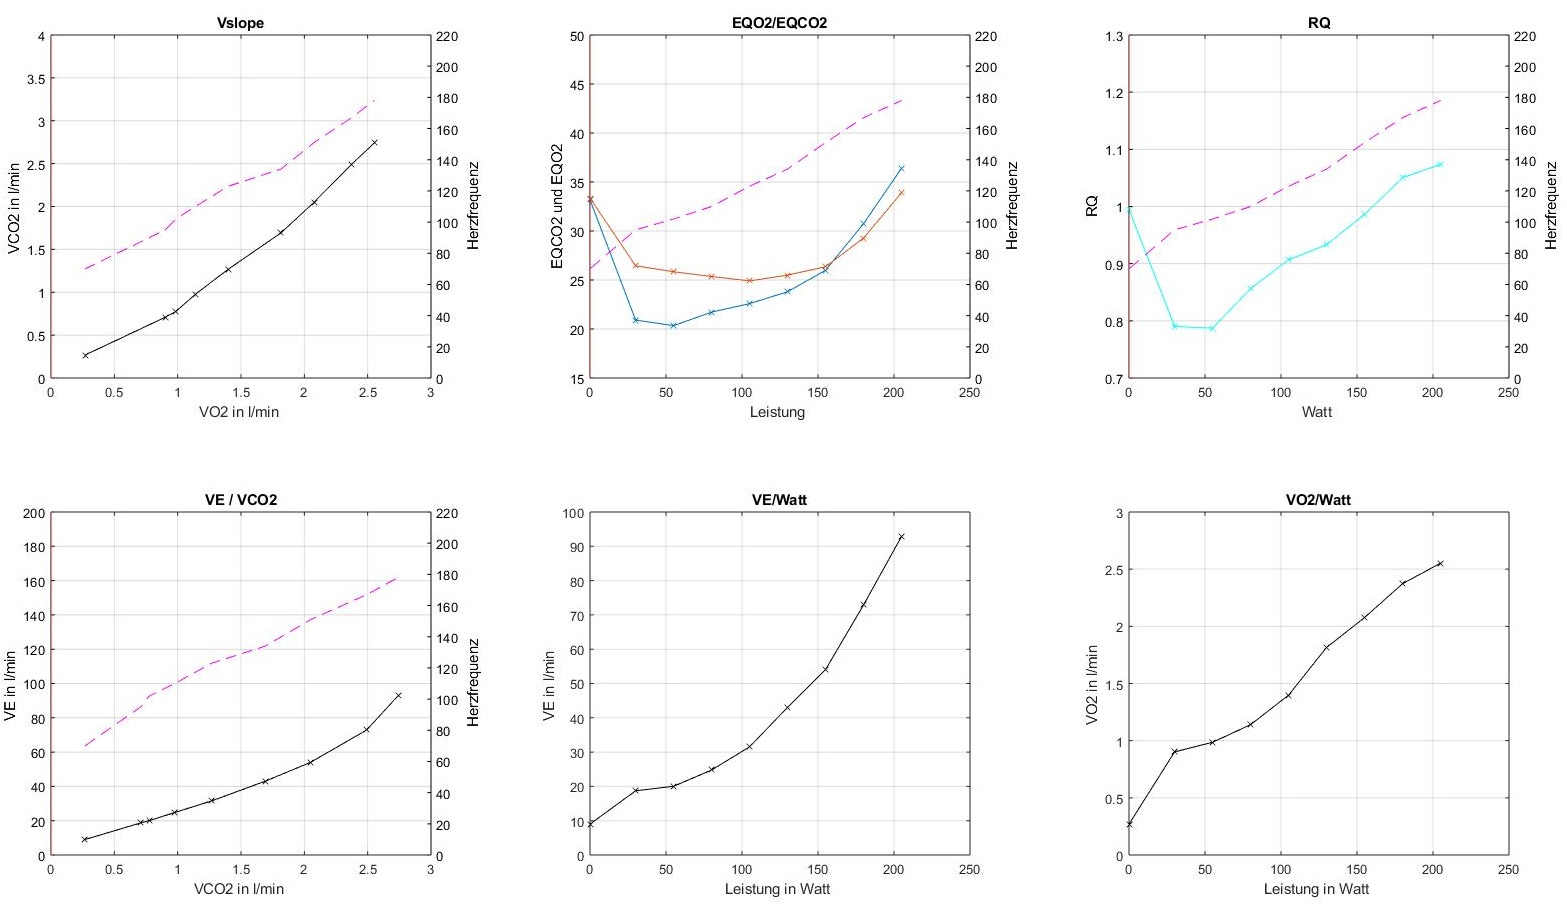
\includegraphics[width=200mm]{Bilder/plot_6w.jpg}}
\put(1.3,1.5){\parbox{720pt}{{\bf \small Abb. 5:} \small Beispiel einer 6-Felder-Grafik}}
\end{picture}
\end{center}

